%!TEX root = paper.tex
\subsection{Statistical learning framework}
We now formally introduce the statistical learning framework adopted to perform joint feature selection and disease prediction with spatial information taken into consideration.

\subsubsection{Regularized empirical risk minimization and feature selection}
In this work, we are interested in the supervised learning problem of linear binary classification.
Suppose we are given a set of training data \sloppy{$\left\{(\x_1,y_1),\cdots,(\x_n,y_n)\right\}$}, where $\x_i\in\reals^p$ is the input feature vector and ${y_i\in\{-1,+1\}}$ is the corresponding class label for each $i\in[n]$.
In our application, $\x_i$ represents functional connectome and $y_i$ indicates the diagnostic status of subject $i\in[n]$, where we adopt the convention of letting $y=+1$ indicate ``disorder'' and $y=-1$ indicate ``healthy'' in this article.
The goal is to learn a linear decision function $\sign{\inprod{\x,\w}}$, parameterized by weight vector $\w\in\reals^p$, that predicts the label $y\in\{-1,+1\}$ of a new input $\x\in\reals^p$.
A standard approach for estimating \w is solving a regularized empirical risk minimization (ERM) problem with the form 
\begin{equation}
	\argmin{\w\in\reals^p} \frac{1}{n} \sum_{i=1}^n \loss\left(y_i \inprod{\w,\x_i}\right) + \lambda\Reg(\w) \;.
	\label{eqn:reg,erm}
\end{equation}
The first term $\frac{1}{n}\sum_{i=1}^n \loss\left(y_i \inprod{\w,\x_i}\right)$ corresponds to the \emph{empirical risk} of a margin-based loss function $\loss:\reals\to\reals_+$ (\eg, hinge, logistic, exponential), which quantifies how well the model fits the data.
The second term $\Reg:\reals^p\to\reals_+$ is a \emph{regularizer} that curtails overfitting and enforces some kind of structure on the solution by penalizing weight vectors that deviate from the assumed structure.
The user-defined regularization parameter $\lambda\geq0$ controls the tradeoff between data fit and regularization. 
Throughout this work, we assume the loss function and the regularizer to be convex, but not necessarily differentiable.
Furthermore, we introduce the following notations 
\[
	\begin{array}{ccc}
		\Y:=\diag{y_1,\cdots,y_n}			, &
		\X:=\ba{c} \x_1^T \\ \vdots \\ \x_n^T \ea , &
		\YXw=\ba{c} y_1 \inprod{\w,\x_1} \\ \vdots \\ y_n \inprod{\w,\x_n} \ea ,
	\end{array}
\]
which allow us to express the empirical risk succinctly by defining a functional \sloppy{${\Loss:\reals^n\to\reals_+}\;$} which aggregates the total loss ${\Loss(\YXw):=\sum_{i=1}^n \loss(y_i \inprod{\w,\x_i})}\,$.

Regularized ERM \eqref{eqn:reg,erm} has a rich history in statistics and machine learning, and many well known estimators can be recovered from this framework.
For example, when the hinge loss ${\loss(t):=\text{max}(0,1-t)}$ is used with the smoothness promoting \elltwo-regularizer $\norm{\w}^2_2$, we recover the SVM \citep{Cortes:1995}.
However, while smoothness helps prevent overfitting, it is problematic for model interpretation, as all the coefficients from the weight vector contribute to the final prediction function.
Automatic feature selection can be done using the \ellone-regularizer $\norm{\w}_1$ known as the Lasso \citep{Tibshirani:1996}, which causes many of the coefficients in \w to be exactly zero.
Because the prediction function is described by a linear combination between the weight \w and the feature vector \x, we can directly identify and visualize the regions that are relevant for prediction.

While the \ellone-regularizer possesses many useful statistical properties, several works have reported poor performance when the features are highly correlated.
More precisely, if there are clusters of correlated features, Lasso will select only a single representative feature from each cluster group, ignoring all the other equally predictive features.
This leads to a model that is overly sparse and sensitive to data resampling, creating problems for interpretation.
To address this issue, \cite{Zou:2005} proposed to combine the \ellone and \elltwo regularizers, leading to the Elastic-net, which has the form $\norm{\w}_1+\frac{\gamma}{2\lambda}\norm{\w}^2_2$, where $\gamma\geq 0$ is a second regularization parameter. 
The \ellone-regularizer has the role of encouraging sparsity, whereas the \elltwo-regularizer has the effect of allowing groups of highly correlated features to enter the model together, leading to a more stable and arguably a more sensible solution.  
While Elastic-net addresses part of the limitations of Lasso and has been demonstrated to improve prediction accuracy \citep{Carroll:2009,Ryali:2010}, it does not leverage the $6$-D structure of connectome space.  To address this issue, we employ the fused Lasso and GraphNet \citep{Grosenick:2013}.

%===================================================================%
% Structured sparsity with spatial information
%===================================================================%
\subsubsection{Spatially informed feature selection and classification via fused Lasso and GraphNet}
The original formulation of fused Lasso \citep{Tibshirani:2005} was designed for encoding correlations among successive variables in $1$-D data, such as mass spectrometry and comparative genomic hybridization (CGH) data \citep{Gui-Bo-Ye:2011}.
More specifically, assuming the weight vector $\w\in\reals^p$ has a natural ordering among its coordinates $j\in[p]$, the regularized ERM problem with the fused Lasso has the following form:
\begin{equation}
	\argmin{\w\in\reals^p}\frac{1}{n}\Loss(\YXw) + \lambda\norm{\Bw}_1 + 
		\gamma\sum_{j=2}^p\abs{w^{(j)} - w^{(j-1)}} \;,
	\label{eqn:fused,lasso,1d}
\end{equation}
where $w^{(j)}$ indicates the $j$-th entry of \w.
Like Elastic-net, this regularizer has two components: the first component is the usual sparsity promoting \ellone-regularizer, and the second component penalizes the absolute deviation among adjacent coordinates.
Together, they have the net effect of promoting sparse and piecewise constant solutions.

The idea of penalizing the deviations among neighboring coefficients can be extended to other situations where there is a natural ordering among the feature coordinates.
For instance, the extension of the $1$-D fused Lasso \eqref{eqn:fused,lasso,1d} for $2$-D imaging data is to penalize the \emph{vertical} and \emph{horizontal} difference between pixels; here, the coordinates are described via lexicographical ordering.
This type of generalization applies to our \mbox{$6$-D} functional connectomes by the virtue of the grid pattern in the nodes, and the ERM formulation reads
\begin{equation}
	\argmin{\w\in\reals^p}\frac{1}{n}\Loss(\YXw) + \lambda\norm{\Bw}_1 + 
		\gamma\sum_{j=1}^p\sum_{k\in\mathcal{N}_j} \abs{\;w^{(j)}-w^{(k)}} \;,
	\label{eqn:fused,lasso,6d}
\end{equation}
where $\mathcal{N}_j$ is the first-order neighborhood set corresponding to coordinate $j$ in \mbox{$6$-D} connectome space.
The spatial penalty $\gamma\sum_{j=1}^p\sum_{k\in\mathcal{N}_j} \abs{\,w^{(j)}-w^{(k)}}$ accounts for the \mbox{$6$-D} structure in the connectome by penalizing deviations among \emph{nearest-neighbor} edges, encouraging solutions that are spatially coherent in the connectome space.
This type of regularizer is known as an anisotropic total variation (TV) penalty in the image processing community \citep{Wang:2008tv}, and an analogous isotropic TV penalty was applied by \cite{Michel:2011} for the application of $3$-D brain decoding.

When the absolute value penalty in the spatial regularizer ${|\,w^{(j)}-w^{(k)}|}$ in \eqref{eqn:fused,lasso,6d} is replaced by the squared penalty $\frac{1}{2}(w^{(j)}-w^{(k)})^2$, we recover the GraphNet model proposed by \mbox{\cite{Grosenick:2013}}:
\begin{equation}
	\argmin{\w\in\reals^p}\frac{1}{n}\Loss(\YXw) + \lambda\norm{\Bw}_1 + 
		\frac{\gamma}{2}\sum_{j=1}^p\sum_{k\in\mathcal{N}_j} \left(w^{(j)}-w^{(k)}\right)^2 \;.
	\label{eqn:graphnet}
\end{equation}
GraphNet also promotes spatial contiguity, but instead of promoting sharp piecewise constant patches, it encourages the clusters to appear in smoother form by penalizing the quadratic deviations among the nearest-neighbor edges (\ie, the coordinates of the functional connectome \x).
We emphasize that the optimization algorithm we propose can be used to solve both fused Lasso~\eqref{eqn:fused,lasso,6d} and GraphNet~\eqref{eqn:graphnet} with very little modification.

To gain a better understanding of the neighborhood set $\mathcal{N}_j$ in the context of our application, let us denote $(x,y,z)$ and $(x',y',z')$ the pair of $3$-D points in the brain that define the connectome coordinate $j$.
Then, the first-order neighborhood set of $j$ can be written precisely as
\footnote{If $(x,y,z)$ or $(x',y',z')$ are on the boundary of the brain volume, then neighboring points outside the brain volume are excluded from $\mathcal{N}_j$.}
\begin{equation}
	\mathcal{N}_j:=
	\braces{
	\begin{array}{l}
			\big(x\pm 1,y,z,x',y',z'\big), \;
			\big(x,y\pm 1,z,x',y',z'\big), \;
			\big(x,y,z\pm 1,x',y',z'\big),\\
			\big(x,y,z,x'\pm 1,y',z'\big), \;
			\big(x,y,z,x',y'\pm 1,z'\big), \;
			\big(x,y,z,x',y',z'\pm 1\big)
	\end{array}}\; .
	\nonumber
\end{equation}
Fig.~\ref{fig,conn,neighbor} provides a pictorial illustration of $\mathcal{N}_j$ in the case of a $4$-D connectome, where the nodes reside in $2$-D space.

There are multiple reasons why fused Lasso and GraphNet are justified approaches for our problem.
For example, fMRI is known to possess high spatio-temporal correlation between neighboring voxels and time points, partly for biological reasons as well as from preprocessing (\eg, spatial smoothing).
Consequently, functional connectomes contain rich correlations among nearby coordinates in the connectome space.
In addition, there is a neurophysiological basis for why the predictive features are expected to be spatially contiguous rather than being randomly dispersed throughout the brain; this point will be  thoroughly discussed in Sec.~\ref{subsec:why,flasso}.
Finally, the spatial coherence that fused Lasso and GraphNet promote helps decrease model complexity and facilitates interpretation.

Letting $\C\in\reals^{e\times p}$ denote the $6$-D \emph{finite differencing matrix} (also known as the \emph{incidence matrix}), the spatial regularization term for both fused Lasso and GraphNet can be written compactly as
\begin{equation}
	\norm{\C\w}_q^q=\sum_{j=1}^p\sum_{k\in\mathcal{N}_j} |\,w^{(j)}-w^{(k)}|^q,\;\;\; q\in\{1,2\} \;,
	\nonumber
\end{equation}
where each row in \C contains a single $+1$ and a $-1$ entry, and $e$ represents the total number of adjacent coordinates in the connectome.
This allows us to write out the regularized ERM formulation for both fused Lasso~\eqref{eqn:fused,lasso,6d} and GraphNet~\eqref{eqn:graphnet} in the following unified form: 
\begin{equation}
	\argmin{\w\in\reals^p} \frac{1}{n}\Loss(\YXw) + \lambda\norm{\w}_1 + \frac{\gamma}{q}\norm{\C\w}^q_q  \; ,\; q\in\{1,2\}\;.
	\label{eqn:costfx}
\end{equation}
We will focus on this matrix-vector representation hereafter, as it is more intuitive and convenient for analyzing the variable splitting framework in the upcoming section.

%************************ Tikz fig ******************************%
\begin{figure}
	{\begin{center}
	\resizebox{0.39\linewidth}{!}{%!TEX root = paper.tex
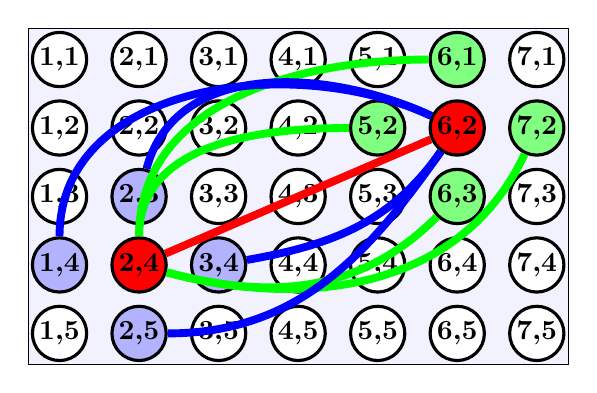
\begin{tikzpicture}[-,red, line width=0.1cm,font=\bfseries,draw=black] 
	\tikzstyle{every node}=[circle,ultra thick,draw=black,fill=white,text=black,minimum size=0cm,line width=0.04cm,inner sep=1pt]
	\tikzstyle{main} =[fill=red]
	\tikzstyle{main1} =[fill=blue!30]
	\tikzstyle{main2} =[fill=green!50]
	\matrix [rectangle,row sep=4pt, column sep=8pt,draw=black,fill=blue!5,line width=0.01cm] % 
	{
	\node  (1_1){1,1} ;& 	\node  (1_2) {2,1} ;&	\node  (1_3) {3,1} ;&	\node  (1_4) {4,1} ;&	\node  (1_5) {5,1} ;&	\node  (MAIN2T)[main2] {6,1}  ;&	\node  (1_7) {7,1} ;\\
	\node  (2_1){1,2} ;& 	\node  (2_2) {2,2} ;&	\node  (2_3) {3,2} ;&	\node  (2_4) {4,2} ;&	\node  (MAIN2L)[main2] {5,2} ;&	\node  (MAIN2)[main] {6,2} ;&	\node  (MAIN2R)[main2] {7,2} ;\\
	\node  (3_1){1,3} ;& 	\node  (MAIN1T)[main1] {2,3} ;&	\node  (3_3) {3,3} ;&	\node  (3_4) {4,3} ;&	\node  (3_5) {5,3} ;&	\node  (MAIN2B)[main2] {6,3} ;&	\node  (3_7) {7,3} ;\\
	\node(MAIN1L)[main1]  {1,4} ;& 	\node  (MAIN1)[main]{2,4} ;&	\node  (MAIN1R)[main1] {3,4} ;&	\node  (4_4) {4,4} ;&	\node  (4_5) {5,4} ;&	\node  (4_6) {6,4} ;&	\node  (4_7) {7,4} ;\\
	\node  (5_1){1,5} ;& 	\node  (MAIN1B)[main1] {2,5} ;&	\node  (5_3) {3,5} ;&	\node  (5_4) {4,5} ;&	\node  (5_5) {5,5} ;&	\node  (5_6) {6,5} ;&	\node  (5_7) {7,5} ;\\
};
	\draw (MAIN1) to (MAIN2) [red];

	\draw[green] (MAIN1) to [out=90,in=180] (MAIN2L) ;
	\draw[green] (MAIN1) to [out=90,in=180] (MAIN2T) ;
	\draw[green] (MAIN1) to [out=-15,in=-115] (MAIN2R) ;
	\draw[green] (MAIN1) to [out=-15,in=-135](MAIN2B) ;
	
	\draw[blue] (MAIN2) to  [out=155,in=90] (MAIN1L) ;
	\draw[blue] (MAIN2) to  [out=155,in=75](MAIN1T) ;
	\draw[blue] (MAIN2) to [out=-125,in=10](MAIN1R) ;
	\draw[blue] (MAIN2) to [out=-125,in=0](MAIN1B) ;
\end{tikzpicture}
}\\
	\textbf{{$\mathcal{N}_j$ in $\bmath{4}$-D Connectome Space}} \vspace{-15pt}\\
	\end{center}	
	}
	\caption{
	Illustration of the neighborhood structure of the connectome when the nodes reside in $2$-D space.  
	The red edge represents coordinate $j=\big\{(2,4),(6,2)\big\}$ in $4$-D connectome space, and its neighborhood set $\mathcal{N}_j$ is represented by the blue and green edges.  
	This idea extends directly to $6$-D connectomes generated from $3$-D resting state volumes.
	}
	\label{fig,conn,neighbor}
\end{figure}
%******************************************************************%
